%-------------------------------------------------------------------------------
% yum_menu
%-------------------------------------------------------------------------------
%
% \file        yum_menu_instruments.tex
% \library     Documents
% \author      Chris Ahlstrom
% \date        2015-05-11
% \update      2016-02-28
% \version     $Revision$
% \license     $XPC_GPL_LICENSE$
%
%     Provides the Menu section of yoshimi-user-manual.tex.
%
%-------------------------------------------------------------------------------

\subsection{Menu / Instruments}
\label{subsec:menu_instrument}

   The \textsl{Yoshimi} Instruments menu lets one select instruments and work
   with banks of instruments.
   \textsl{Yoshimi} stamps instrument XML files with its own major and minor
   version numbers so it is possible to tell which version created the files,
   or whether they were created by \textsl{ZynAddSubFX}.

   When opening an instrument bank one can now tell exactly which synth engines
   are used by each instrument. This is represented by three pale background
   colours:

   \begin{itemize}
      \item \textcolor{red}{Red}: ADDsynth
      \item \textcolor{blue}{Blue}: SUBsynth
      \item \textcolor{green}{Green}: PADsynth
   \end{itemize}

   These new colored engine backgrounds aren't just pretty. They give real
   information about expected processor load, and time taken to be ready when
   loaded:

   \begin{itemize}
      \item \textsl{Processor Load, low to high}: PAD, SUB, then ADD.
      \item \textsl{Time to initialize, low to high}: SUB, ADD, PAD.
   \end{itemize}

   If the instruments are kits they scanned to find out if 
   \textsl{any} member of the kit contains each engine.
   This scanning is duplicated in the current part, the mixer panel for the
   currently loaded instruments, and in the Instrument Edit window the same
   colors highlight the engine names when they are enabled with the check
   boxes. 

   The following sub-menus are provided, as shown in
   \figureref{fig:yoshimi_instrument_menu}.

\begin{figure}[H]
   \centering 
   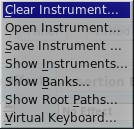
\includegraphics[scale=1.0]{1.3.8/yoshimi-menu-instrument.jpg}
   \caption{Yoshimi Menu, Instrument}
   \label{fig:yoshimi_instrument_menu}
\end{figure}

   TODO:  Document the many differences in 1.3.8 here.

   \begin{enumber}
      \item \textbf{Clear Instrument...}
      \item \textbf{Open Instrument...}
      \item \textbf{Save Instrument...}
      \item \textbf{Show Instruments...}
      \item \textbf{Show Banks...}
      \item \textbf{Show Root Paths...}
   \end{enumber}

   These menu entries don't appear in the order in which they would normally
   be used.  For simplicity, it is better, especially for \textsl{Yoshimi}
   1.3.5 and above, to summarize how to navigate through these menu items,
   before showing each one in detail.

   \setcounter{ItemCounter}{0}      % Reset the ItemCounter for this list.

   \itempar{Set Current Root Path}{root!set current}
   \index{root!current}
   Instruments are stored in banks, and banks are stored in root directories,
   also known as "roots".  In \textsl{Yoshimi}, there can be a number of
   roots that exist in a user's directory structure, but only one root can be
   the current root.  Thus, the first step is to set up the current root
   directory to point to where we have stored all our banks of instruments.

   \begin{enumber}
      \item In \textsl{Yoshimi}, navigate to the \textbf{Instrument / Show
      Root Paths...} entry in the main menu.
      \item In the \textbf{Bank Root Paths} dialog, select the desired
      bank path by clicking on it.
      \item Click the \textbf{Make Current} button.
%     \item Then click the \textbf{Open Current} button.
      \item Then click the \textbf{Save and Close} button.
   \end{enumber}

   For example, one can make the \texttt{/usr/share/yoshimi/banks} directory
   the current root directory.  This directory is the default location for
   banks when \textsl{Yoshimi} is first installed.
   In the following figure, we set it to the author's local directory,
   \texttt{~/Audio/yoshimi/banks}.
   In general, it is recommended that one copies the default installed
   directories to a local directory, in order to be able to work with them,
   making additions and changes without needing root permissions, and
   without risking the corruption of the default installation.

   For figures and details about the \textbf{Show Root Paths...} menu entry,
   see \sectionref{subsubsec:menu_instrument_show_root_paths}.

   \itempar{Show Current Bank Set}{banks!show}
   Once the current root has been set, one can then see all of the banks
   under that root.  Navigate to the \textbf{Instrument / Show Banks...} menu
   entry and click it.  This brings up a dialog such as the one shown in
   \figureref{fig:show_ca_banks}.
   That dialog shows all of the banks that
   exist in the current root directory.  Each is auto-numbered by
   \textsl{Yoshimi} the first time that root directory is accessed, and the
   current bank is highlighted in pink.

   Clicking on a bank with both make that bank the current bank, and opens an
   instruments dialog, such as that shown in
   \figureref{fig:show_alex_j_bank}.

   \itempar{Show Instruments in Current Bank}{instruments!show}
   Once the current root and current bank have been set, another way to show
   the instruments is to navigate to the
   \textbf{Instrument / Show Instruments...} menu entry and click on it.
   Again, this action opens an instruments dialog, such as that shown in
   \figureref{fig:show_alex_j_bank}.

   A left-click on a particular instrument sets that instrument into the
   current Part in force in the main \textsl{Yoshimi} window, where it can
   then be edited, if desired.

   \index{anti-auto-clutter}
   Right-clicking on an instrument causes the instruments list dialog
   to disappear, and be replaced by an instrument dialog.  While this
   behavior might be surprising, it is part of the anti-auto-clutter feature
   of \textsl{Yoshimi}.

   Now that we know how to easily navigate through roots, banks, and
   instruments, we can discuss each of the \textbf{Instrument} menu entries
   in detail.

\subsubsection{Menu / Instrument / Clear Instrument...}
\label{subsubsec:menu_instrument_clear}

   This menu entry brings up a prompt to clear the parameters of the
   instrument that is currently loaded in the current part.

\begin{figure}[H]
   \centering 
   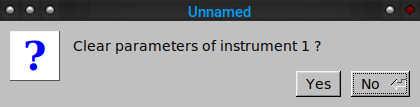
\includegraphics[scale=0.75]{menu/Instrument/clear-instrument.jpg}
   \caption{Clear Instrument Dialog}
   \label{fig:clear_instrument_dialog}
\end{figure}

   \textbf{Bug:}
   \index{bugs!need to clear instrument?}
   Sometime it seems that one needs to clear the instrument if one is
   loading a new instrument to test it out, because some settings seem
   to remain from the previous instrument.

   \textsl{Don't quote us on that.  Maybe Will has fixed that issue by now.}

\subsubsection{Menu / Instrument / Open Instrument...}
\label{subsubsec:menu_instrument_open}

   This menu entry brings up a prompt to open a new instrument.
   This prompt is a file-dialog, and it doesn't depend at all on the settings
   of the current root or the current bank.  It does have a
   \textbf{Favorites} button to help the user get quickly to the desired
   location of instrument files.

\begin{figure}[H]
   \centering 
   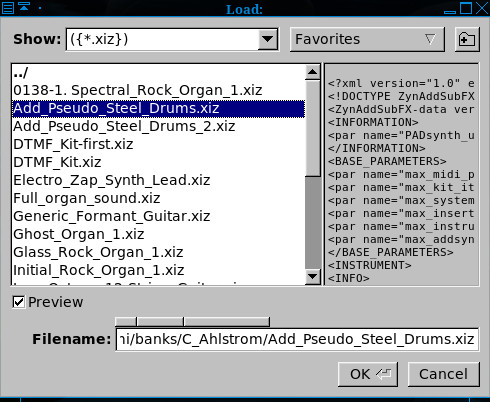
\includegraphics[scale=0.75]{menu/Instrument/open-instrument.jpg}
   \caption{Open Instrument Dialog}
   \label{fig:open_instrument_dialog}
\end{figure}

   This dialog has a number of user-interface elements to discuss.

   \begin{enumber}
      \item \textbf{Show}
      \item \textbf{Favorites}
      \item \textbf{Create a new diretory}
      \item \textbf{Instrument List}
      \item \textbf{XML Preview}
      \item \textbf{Preview}
      \item \textbf{Show hidden files}
      \item \textbf{Directory Bar}
      \item \textbf{Filename}
      \item \textbf{OK}
      \item \textbf{Cancel}
   \end{enumber}

   \setcounter{ItemCounter}{0}      % Reset the ItemCounter for this list.

   \itempar{Show}{Open Instrument!show}
   Show types of files.
   This item shows a file filter for selecting instrument files.
   The types of filters are as follows (screen shot not available):

   \begin{enumber}
      \item \textbf{(\{*.xiz\})} (compressed XML files)
      \item \textbf{All Files (*)}
      \item \textbf{Custom Filter}
   \end{enumber}

   \itempar{Favorites}{Open Instrument!favorites}
   Favorite directories.
   Provides a list of options and favorite directories in which to find 
   instrument files.

\begin{figure}[H]
   \centering 
   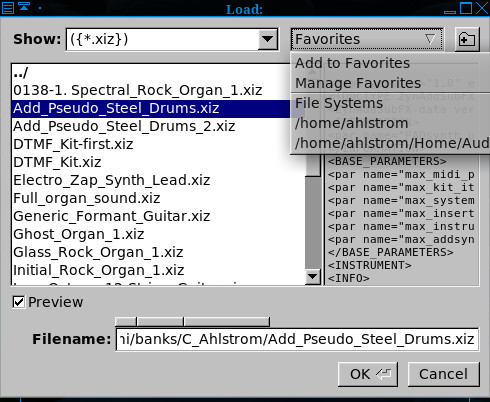
\includegraphics[scale=0.75]{menu/Instrument/favorites-dropdown.jpg}
   \caption{Favorites Drop-down}
   \label{fig:open_instrument_favorites}
\end{figure}

   \begin{enumber}
      \item \textbf{Add to Favorites}
      \item \textbf{Manage Favorites}
      \item \textbf{File Systems}
      \item \textbf{(Additional favorite directories)}
   \end{enumber}

   \index{Add to Favorites}
   \textbf{Add to Favorites}
   simply adds the currently selected directory shown in the instrument list
   to the list of favorites.

   To add Favorites in the file dialog, navigate to the desired directory.
   Then click \textbf{Favorites}, and select \textbf{Add to Favorites}.

   Once one has a number of favorites set up,
   there is a \textbf{Manage Favorites} that can be used.
   For example, if one needs to get rid of a directory, one can use the
   \textbf{Manage Favorites}
   \index{Manage Favorites}
   dialog, shown in
   \figureref{fig:manage_instrument_favorites}, below to do that.

\begin{figure}[H]
   \centering 
   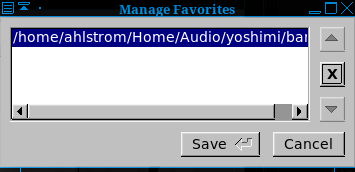
\includegraphics[scale=1.0]{menu/Instrument/manage-favorites.png}
   \caption{Favorites Drop-down}
   \label{fig:manage_instrument_favorites}
\end{figure}

   \textbf{File Systems} \index{File Systems}
   Provides a list of all file systems starting at root ("\texttt{/}").
   This list can be pretty confusing, with a lot of entries.
   But note that one navigates to ("\texttt{/}"), and from there to
   \texttt{/usr/share/yoshimi/banks} to get easy access to all the
   instruments that are preinstalled with
   \textsl{Yoshimi}.
   Generally, one will want to use only
   \textbf{Add to Favorites} and \textbf{Manage Favorites}.

   \itempar{Create Directory}{Open Instrument!create new directory}
   Creates a New Directory.
   This little symbol options a small "New Directory?" dialog (not shown
   here, it is very simple and stock) into which one can type a directory
   name to be added to the current directory of the instrument list.

   \itempar{Instrument List}{Open Instrument!instrument list}
   Provides a list of the instrument files available in the current
   directory.  Also shown are sub-directories (if available)
   that might contain more instruments, and a ("\texttt{../}") entry
   to navigate to the parent directory.

   \itempar{Preview}{Open Instrument!preview checkbox}
   If one thinks the preview feature is not useful, uncheck this check-box.
   so that one doesn't see the preview window.  As a bonus, one can see more
   of the instrument file-name.

   \itempar{Preview pane}{Open Instrument!preview pane}
   XML Preview.
   This box can show the beginning of the XML data of an instrument file.
   \textbf{Bug:}
   \index{bugs!compressed XML preview}
   It seems to show the XML only if the XML is not compressed.

   \itempar{Show hidden files}{Open Instrument!show hidden files}
   Shows file that are hidden.  Not sure how useful this feature is;
   who would hide a \textsl{Yoshimi} instrument file?

   \itempar{Directory Bar}{Open Instrument!directory bar}
   Provides an alternate way to move up through the directory structure.

   \itempar{Filename}{Open Instrument!filename}
   File Name.
   Provides the full path to the instrument file.

   \itempar{OK/Cancel}{Open Instrument!ok/cancel}
   We don't really need to discuss the \textbf{OK} and \textbf{Cancel}
   buttons, do we?

\subsubsection{Menu / Instrument / Save Instrument...}
\label{subsubsec:menu_instrument_save}

   This menu entry brings up a prompt to save a new instrument within the
   user's file system.
   It has all of the user-interface elements of the "Open Instrument"
   dialog shown in
   \figureref{fig:open_instrument_dialog},
   in \sectionref{subsubsec:menu_instrument_open}.
   Like that dialog, it is not dependent on the current root or current bank.
   However, if nothing has changed, then a "Nothing to Save!" prompt (not
   pictured) is shown.

   With \textsl{ZynAddsubFX} and older versions of \textsl{Yoshimi},
   it was possibly to end up with unnamed instruments. Since version
   1.3.4, \textsl{Yoshimi} will trap such an occurrence and name it
   'No Title'; it will not let one save the unedited default sound.

\subsubsection{Menu / Instrument / Show Instruments...}
\label{subsubsec:menu_instrument_show}

   Instruments are stored in banks. The banks (and current bank setting)
   are loaded/saved
   automatically by the program, so one doesn't have to worry about saving the
   banks before the program exits. On program start, the last used bank is
   loaded. A single bank can store up to 128 instruments. 
   However, there is space for a number of additional
   instruments in the bank, the extended-program section, to allow up to 160
   instruments in a bank.

   When the \textbf{Show Instruments...} button is selected, a dialog comes
   up that shows all of the instruments present in the currently-selected
   bank.
   
\begin{figure}[H]
   \centering 
   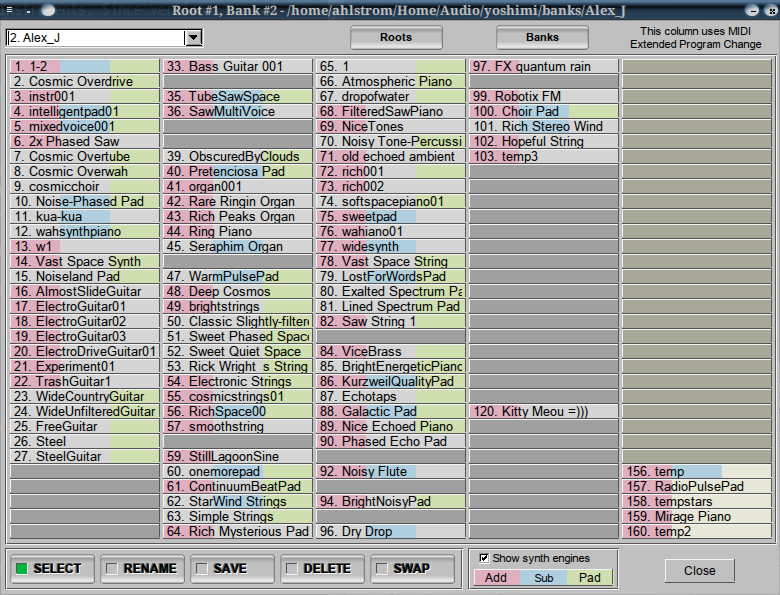
\includegraphics[scale=0.75]{1.3.6/Alex_J_bank_instruments.png}
   \caption[Instruments in Current Bank]{Instruments in Current Bank 1.3.6}
   \label{fig:show_alex_j_bank}
\end{figure}

   As \figureref{fig:show_alex_j_bank}
   shows, this is a very complex dialog with a lot of options.
   Note how \textsl{Yoshimi} now shows the color codings for the
   synth-sections used in each instrument:
   red for ADDsynth, blue for SUBsynth, and
   green for PADsynth.

   Also note how the numbers at the beginning of the filenames are used as
   an "instrument" or "program" number.  These numbers can be used in MIDI
   Program Change commands.
   
   All of the files with filenames starting with 4-digit numbers will be
   shown in the slot corresponding number.  Those without numbers will start
   with numbers at 129 or above ("extended program change").  One should give
   them numbers by renaming them outside of \textsl{Yoshimi}, then reloading
   the bank.

   \index{extended program}
   Note that MIDI CC
   (see \sectionref{paragraph:menu_yoshimi_settings_ccs})
   can be set to access voices from 129 to 160.
   All the Bank controls in the \textbf{MIDI} settings tab take immediate
   effect when set.
   Bank and program changes can be completely disabled in the settings tab;
   some hardware synths don't play nice with it.

   Learning how to use the Instruments dialog is an important way to make
   instruments easier to manage, and so this will be a long discussion.

%  An important pair of concepts in \textsl{Yoshimi} are
%  \textsl{banks} and \textsl{roots}.  These concepts are described in
%  \sectionref{subsec:concepts_banks_and_roots}.

%  A bank has 3 modes in \textsl{ZynAddSubFX}: 

%  \begin{enumber}
%     \item \textbf{READ}.
%        The instrument is loaded from the bank to the current part.
%     \item \textbf{WRITE}.
%        The instrument is written to the bank.
%     \item \textbf{CLEAR}.
%        The instrument from the bank is cleared (removed).
%  \end{enumber}

%  Pressing the left mouse button on a slot reads/writes/clears the
%  instrument from/to it (according to the current mode).
   
%  Pressing the right mouse button on a slot changes its name.

%  The setup in \textsl{Yoshimi} is a bit different than in
%  \textsl{ZynAddSubFX}.
%  Observe \figureref{fig:show_ca_bank}.
%  It shows a bank loaded from a directory containing customs
%  banks from one of the authors of this document.

   Note that this dialog has been modified in recent versions of
   \textsl{Yoshimi}.

   Here is a list of the user-interface items in the instruments/banks dialog.

   \begin{enumber}
      \item \textbf{Bank Names}
      \item \textbf{Roots}
      \item \textbf{Banks}
      \item \textbf{Instrument and Bank Matrix}
      \item \textbf{SELECT}
      \item \textbf{RENAME}
      \item \textbf{SAVE}
      \item \textbf{DELETE}
      \item \textbf{SWAP}
      \item \textbf{Show synth engines}
         (was \textbf{Show PADsynth status})
      \item \textbf{Close}
   \end{enumber}

   \setcounter{ItemCounter}{0}      % Reset the ItemCounter for this list.

   \itempar{Bank Names}{instruments!bank names}
   Instruments Bank Name.
   Basically, each bank is a directory name, with a number prepended.
   The banks are found under the current root, which is a also a directory
   name, and is the name of the parent directory of a set of banks.
   Here is the Bank Names drop-down list for "my" setup, which has the
   default banks plus a lot of banks found around the Internet:

\begin{figure}[H]
   \centering 
   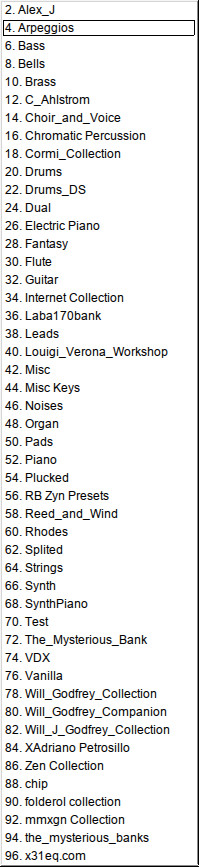
\includegraphics[scale=0.75]{menu/Instrument/bank-list.jpg}
   \caption[A Sample Bank List]{A Sample Bank List}
   \label{fig:bank_list}
\end{figure}

   And here is the directory listing associated with it, in the order
   produced by the UNIX/Linux "ls -1" (list single-column) command (shown in
   two columns to save space):

   \begin{verbatim}
      Alex_J                        Noises
      Arpeggios                     Organ
      Bass                          Pads
   '  Bells                         Piano
      Brass                         Plucked
      C_Ahlstrom                    RB Zyn Presets
      chip                          README
      Choir_and_Voice               Reed_and_Wind
      Chromatic Percussion          Rhodes
      Cormi_Collection              Splited
      Drums                         Strings
      Drums_DS                      Synth
      Dual                          SynthPiano
      Electric Piano                Test
      Fantasy                       The_Mysterious_Bank
      Flute                         the_mysterious_banks
      folderol collection           Vanilla
      Guitar                        VDX
      Internet Collection           Will_Godfrey_Collection
      Laba170bank                   Will_Godfrey_Companion
      Leads                         Will_J_Godfrey_Collection
      Louigi_Verona_Workshop        x31eq.com
      Misc                          XAdriano Petrosillo
      Misc Keys                     Zen Collection
      mmxgn Collection
   \end{verbatim}

   The first thing to note is that there are only 128 \textsl{Yoshimi} banks
   supported in a \textsl{Yoshimi} root.  The list above takes up about half
   of the available slots, so it might be time to move some of those banks
   to a new root directory.

   The numbers in the drop-down list are generated by \textsl{Yoshimi} the
   first time it sees a new root path or a new bank within the root path.
   Once set, these numbers will never change unless one actually moves them
   around (using the \textbf{SWAP} button).

   The bank number is also the MIDI ID for the bank;
   one can be sure that it will always
   be there for bank changes, no matter how many banks are added later.
   \textsl{Yoshimi} always lists the banks in ID order, not alphabetical
   order, so one can group them sensibly and permanently.
   However, at first-time creation \textsl{Yoshimi} sets the IDs in
   alphabetical order and tries to space them evenly over the range to
   provide some wiggle room.                                        

   Selecting one of the items in this drop-down list selects the bank and
   loads it into the Banks dialog.

   \index{anti-auto-clutter}
   Right-clicking on a bank causes the banks list dialog
   to disappear, and be replaced by the bank dialog.  While this
   behavior might be surprising, it is part of the anti-auto-clutter feature
   of \textsl{Yoshimi}.

   \itempar{Roots}{instruments!roots}
   Instruments Roots Button.
   Shows a list of directories that can serve as "root" directories.
   The "Bank Root Paths" dialog shown in
   \figureref{fig:show_banks_roots} shows
   the system root (e.g. \texttt{/usr/share/yoshimi/banks}) and
   a user's home location for his/her banks and roots.

   \itempar{Banks}{instruments!banks}
   Banks Button.
   This item brings up a Banks dialog showing all of the banks present in the
   current root.
   It is an alternative to using the \textbf{Bank Names} dropdown list.

   \itempar{Instrument and Bank Matrix}{instruments!bank matrix}
   Instruments Bank Matrix.
   Shows the instruments that are in the currently selected bank
   (directory).

   \itempar{SELECT}{instruments!SELECT}
   Instruments SELECT.
   When this button is selected, then clicking on an instrument selects that
   instrument as the instrument for the current Part active in the main
   window.

   \itempar{RENAME}{instruments!RENAME}
   Instruments RENAME.
   When this button is selected, then clicking on a bank brings
   up a small dialog to rename the clicked-on bank.
   However, one might also experience the following warning message:

   \begin{verbatim}
      This instrument file cannot be changed
   \end{verbatim}

   \itempar{SAVE}{instruments!SAVE}
   Instruments SAVE.
   When this button is selected, then clicking on a bank saves
   the instruments as currently configured.
   However, one might also experience the following warning message:

   \begin{verbatim}
      This instrument file cannot be changed
   \end{verbatim}

   \itempar{DELETE}{instruments!DELETE}
   Instruments DELETE.
   Selecting this button and clicking an empty bank entry does nothing.
   Selecting this button and clicking an existing bank entry brings up a
   small dialog asking one if this bank is really to be deleted.
   However, one might also experience the following warning message:

   \begin{verbatim}
      This instrument file cannot be changed
   \end{verbatim}

   \itempar{SWAP}{instruments!SWAP}
   Instruments SWAP.
   Selecting this button, then selecting one bank, and then another,
   swaps the numbering and postion of the selected banks.
   However, one might also experience the following warning message:

   \begin{verbatim}
      This instrument file cannot be changed
   \end{verbatim}

   \itempar{Show synth engines}{instruments!show engines}
   If enabled, then the usage of each of the \textsl{Yoshimi} synthesis
   engines is indicated by color coding, as shown in the figure above.

   \itempar{Close}{instruments!Close}
   Closes the window.

   Here is a more conventional view of instruments, supplied with
   \textsl{Yoshimi}, shown in
   \figureref{fig:show_pads_bank}.

\begin{figure}[H]
   \centering 
%  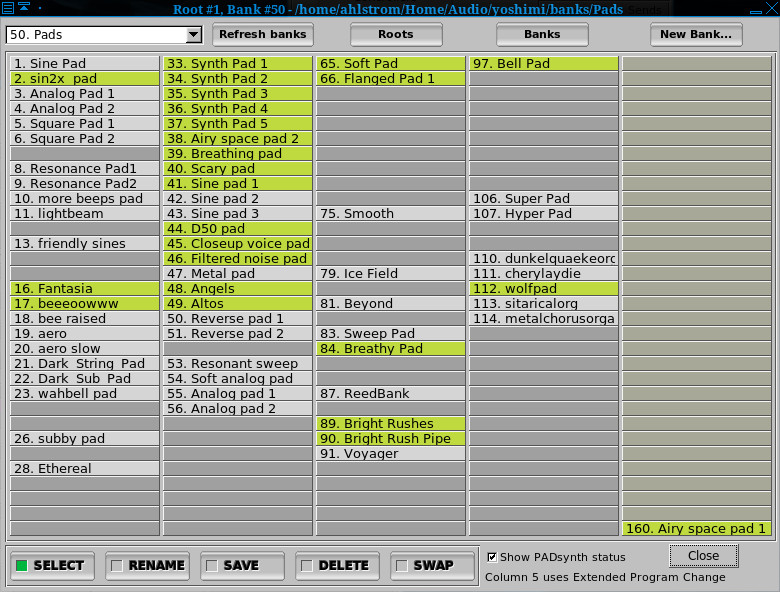
\includegraphics[scale=0.75]{menu/Instrument/show-pads-bank.jpg}
   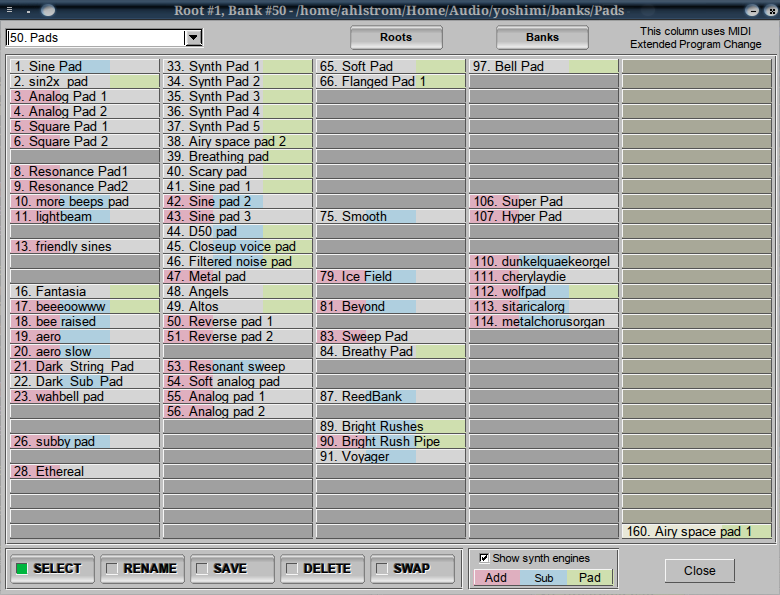
\includegraphics[scale=0.75]{1.3.6/show_pads_bank.png}
   \caption[Show Pads Instruments]{Show Pads Instruments}
   \label{fig:show_pads_bank}
\end{figure}

   Note that many of these Pads instruments also use the Add and Sub
   components as well.

\subsubsection{Menu / Instrument / Show Banks...}
\label{subsubsec:menu_instrument_show_banks}

   This menu entry brings up a dialog that shows all of the banks present in
   the current root.

\begin{figure}[H]
   \centering 
   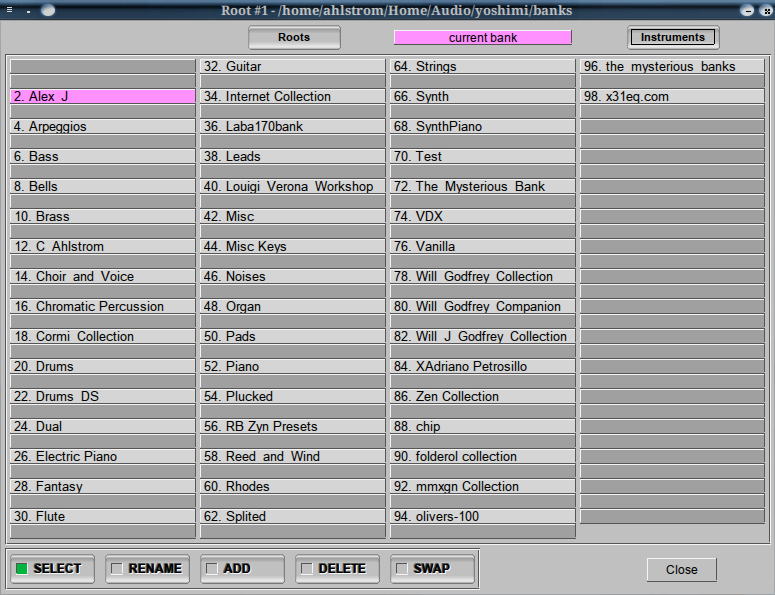
\includegraphics[scale=0.75]{1.3.6/show_CA_banks.png}
   \caption[Show Banks]{Show Banks in Current Root}
   \label{fig:show_ca_banks}
\end{figure}

   This figure illustrates a setup where the installed banks were combined with
   banks downloaded from various web sites.
   The following list shows that the interface elements in the banks dialog
   are slightly different from the instruments dialog.

   \begin{enumber}
      \item \textbf{Roots}
      \item \textbf{Current Bank} (passive display element)
      \item \textbf{Instruments}
      \item \textbf{SELECT}
      \item \textbf{RENAME}
      \item \textbf{ADD}
      \item \textbf{DELETE}
      \item \textbf{SWAP}
      \item \textbf{Close}
   \end{enumber}

   \setcounter{ItemCounter}{0}      % Reset the ItemCounter for this list.

   \itempar{Roots}{banks!roots}
   Banks Roots.
   "Roots" button.
   Shows a list of directories that can serve as "root" directories.

   \itempar{current bank}{banks!current bank}
   \index{current!bank}
   Current Bank.  Simply indicates the current bank via color-highlighting.
   Note that one can left-click on a bank in this dialog to make it the
   current bank.  This setting is saved across \textsl{Yoshimi} restarts.

   \itempar{Instruments}{banks!instruments}
   Banks Instruments.
   \index{current!bank}
   Brings up a banks dialog that shows the instruments in the current bank.

   \itempar{SELECT}{banks!SELECT}
   Banks SELECT.
   When this button is selected, then clicking on a bank makes it the current
   bank.

   (Although we don't show a figure for it, note that some banks provide
   instruments with numbers in the extended program-change range (above
   127) prepended to the file-names.)

   \itempar{RENAME}{banks!RENAME}
   Banks RENAME.
   When this button is selected, then clicking on a bank brings
   up a small dialog to rename the clicked-on bank.
   However, one might also experience the following warning message:

   \begin{verbatim}
      This bank directory cannot be changed
   \end{verbatim}

   \itempar{ADD}{banks!ADD}
   Banks ADD.
   Selecting this button and clicking an empty bank entry brings up a small
   dialog to create a new empty bank name for that entry.
   If one clicks on an existing bank entry, then a small dialog comes up
   stating that the bank number selected is already in use.
   However, one might also experience the following warning message:

   \begin{verbatim}
      This bank directory cannot be changed
   \end{verbatim}

   \itempar{DELETE}{banks!DELETE}
   Banks DELETE.
   Selecting this button and clicking an empty bank entry does nothing.
   Selecting this button and clicking an existing bank entry brings up a
   small dialog asking one if this bank is really to be deleted.
   However, one might also experience the following warning message:

   \begin{verbatim}
      This bank directory cannot be changed
   \end{verbatim}

   \itempar{SWAP}{banks!SWAP}
   Banks SWAP.
   Selecting this button, then selecting one bank, and then another,
   swaps the numbering and postion of the selected banks.
   This button is good for minor reorganization of the bank numbers.

\subsubsection{Menu / Instrument / Show Root Paths...}
\label{subsubsec:menu_instrument_show_root_paths}

\begin{figure}[H]
   \centering 
   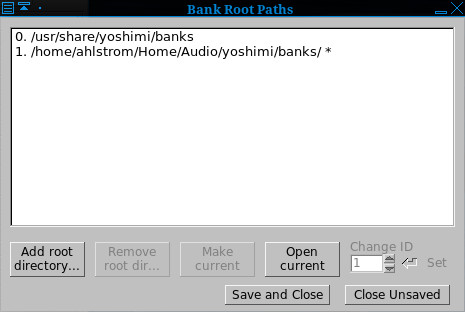
\includegraphics[scale=0.75]{menu/Instrument/show-banks-roots.jpg}
   \caption[Show Root Paths]{Show Root Paths}
   \label{fig:show_banks_roots}
\end{figure}

   \setcounter{ItemCounter}{0}      % Reset the ItemCounter for this list.

   \itempar{Add root directory...}{Root Paths!add directory}
   Show Root Paths Add Root Directory.
   To add a bank root path:

   \textsl{Yoshimi} (as installed by Debian Linux) provides a default bank at
   \texttt{/usr/share/yoshimi/banks}.
   To add one's own directory, navigate to "Yoshimi / Instrument / Show Root
   Paths ...".  Then click on "Add root directory...".

   Once selected, one will see that \texttt{/usr/share/yoshimi/banks}
   is marked with an asterisk.  One can select the new root directory,
   and make it current by clicking the "Make current" button.
   Then the Banks dialog will show all the banks in that directory, one bank
   per subdirectory (each subdirectory "is" a bank).

\begin{figure}[H]
   \centering 
   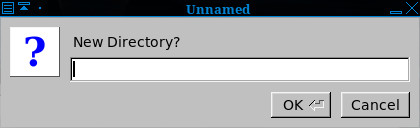
\includegraphics[scale=0.75]{menu/Instrument/new-directory.jpg}
   \caption{Add Root Directory}
   \label{fig:add_root_directory}
\end{figure}

   \itempar{Remove root directory...}{Root Paths!remove directory}
   Show Root Paths Remove Root Directory.
   If a path is selected, then this button is active, and can be used to
   delete the selected path from the "root paths" list.

   \itempar{Make current}{Root Paths!make current}
   Show Root Paths Make Current.
   \index{current!root}
   This button marks the currently-selected path as the "current root" path.

   \itempar{Open current}{Root Paths!open current}
   Show Root Paths Open Current.
   This button opens the current root path.

   \itempar{Change ID}{Root Paths!change ID}
   Show Root Paths Change ID.

   Values: \texttt{0* to 127}

   \textsl{
   We need to know more about how this ID can be used.
   Is it a way to make the path selectable via an extended MIDI control, or
   some other automation method?
   }

%-------------------------------------------------------------------------------
% vim: ts=3 sw=3 et ft=tex
%-------------------------------------------------------------------------------
